% Template for ISBI-2018 paper; to be used with:
%          spconf.sty  - ICASSP/ICIP LaTeX style file, and
%          IEEEbib.bst - IEEE bibliography style file.
% --------------------------------------------------------------------------
\documentclass{article}
\usepackage{spconf,amsmath, amssymb, graphicx}

% Example definitions.
% --------------------
\def\x{{\mathbf x}}
\def\L{{\cal L}}

% Allow easy processing of labeled images in figures
\newcounter{lfigcounter}
\def\ionbox#1{\makebox[#1]{(\alph{lfigcounter})}\stepcounter{lfigcounter}}
%

% Title.
% ------
\title{Application of Vectorized Persistence Homology Representations for 
Cancer Grading in Histopathology Images}
%
% Single address.
% ---------------
\name{Author(s) Name(s)\thanks{Thanks to XYZ agency for funding.}}
\address{Author Affiliation(s)}
%
% For example:
% ------------
%\address{School\\
%	Department\\
%	Address}
%
% Two addresses (uncomment and modify for two-address case).
% ----------------------------------------------------------
%\twoauthors
%  {A. Author-one, B. Author-two\sthanks{Thanks to XYZ agency for funding.}}
%	{School A-B\\
%	Department A-B\\
%	Address A-B}
%  {C. Author-three, D. Author-four\sthanks{The fourth author performed the work
%	while at ...}}
%	{School C-D\\
%	Department C-D\\
%	Address C-D}
%
% More than two addresses
% -----------------------
% \name{Author Name$^{\star \dagger}$ \qquad Author Name$^{\star}$ \qquad Author Name$^{\dagger}$}
%
% \address{$^{\star}$ Affiliation Number One \\
%     $^{\dagger}$}Affiliation Number Two
%
\begin{document}
%\ninept
%
\maketitle
%
\begin{abstract}
% 100 - 150 words

\end{abstract}
%
\begin{keywords}
Histopathology, Cancer Diagnosis, Cancer Grading, Persistence homology, Persistence diagrams, Persistence images, Persistence landscapes, Machine learning
\end{keywords}
%
\section{Introduction}
\label{sec:intro}
Cancer grading refers to the process of determining the degree of malignancy and is one of the primary criteria used in clinical practice to inform prognosis and plan the treatment of individual patients. However, achieving good reproducibility in grading most cancers remains one of the challenges in pathology practice.

\section{Method}
\label{sec:method}
In this section, we present the theory underlying the proposed method along with visual illustrations of intermediate results to help understand the underlying concepts. In section~\ref{sec:method:homology}, we present a brief background on persistence homology. In section~\ref{sec:method:proposed}, we describe our strategy of using vectorized representations of persistence homology information for cancer grading.

\subsection{Background on persistence homology}
\label{sec:method:homology}
% introduce persistence homology, persistence diagrams
% talk about representational inconvenience of persistence diagrams for ML
% talk about persistence images
% talk about persistence landscapes
% describe how we apply them for cancer diagnosis and grading
Given a dataset representable in the form of a point cloud in some space, persistence homology can be seen as a theoretical tool to detect and characterize its prominent topological features (e.g. connected components, loops, voids) at multiple scales~\cite{Zhu2013PersistentProcessing.}. These topological descriptors can then be used as features for building machine learning models to solve predictive problems. 

The basic building blocks of persistence homology are simplices, simplicial complexes, and homology groups. A p-simplex $\sigma_p$ is defined as the convex hull of $p+1$ affinely independent points/vertices. For example, a single vertex is called a 0-simplex, an edge is called a 1-simplex, a triangle is called a 2-simplex, a tetrahedron is called a 3-simplex, and so on. A face of a p-simplex is defined as a subset of its $p+1$ points/vertices. For example, the tetrahedron which is a 3-simplex has 4 triangular faces, 6 edge faces, and 4 vertex faces each of which are simplices themselves. A simplicial complex $K$ is a finite collection of simplices subject to two conditions: (i) if a simplex $\sigma$ is in $K$ and any face of $\sigma$ is also in $K$, and (ii) if two simplices $\sigma$ and $\sigma'$ are in K then $\sigma \cap \sigma'$ must either be empty or a face of both $\sigma$ and $\sigma'$ i.e. they must either be glued together along whole faces or be separate. A d-dimensional homology group $H_d(K)$ of a simplicial complex $K$ is the set of all d-dimensional holes in it. For example, the 0-dimensional homology group $H_0(K)$ is the set of all connected components, the 1-dimensional homology group $H_1(K)$ is the set of all 2D loops, the 2-dimensional homology group $H_2(K)$ is the set of all 3D cavities and so on. The rank or the number of holes in a d-dimensional homology group $H_d(K)$ is referred to as the d-dimensional Betti number $\beta_d(K)$. 

Given a dataset in the form of a point cloud of $n$ points $x_1, x_2, ..., x_n \in \mathbb{R}^d$, how can we derive a simplicial complex that encodes the underlying topological structure? One approach for generating it is to examine all subsets of $p+1$ points, and add the p-simplex made up of those points to the simplical complex if the distance between all pairs of points in the simplex is less than a present distance $\epsilon$. Such a complex is called a Vectoris-Rips complex of diameter $\epsilon$ which we will henceforth denote as $VR(\epsilon)$. Note that, if a simplex is in $VR(\epsilon)$, then all its faces are also in $VR(\epsilon)$. The schematic below shows the Vectoris-rips complex for different diameters for a dataset of four points corresponding to the corners of a rectangle with width = 2 and height = 1.
%
\begin{figure}[!h]
\centering
%
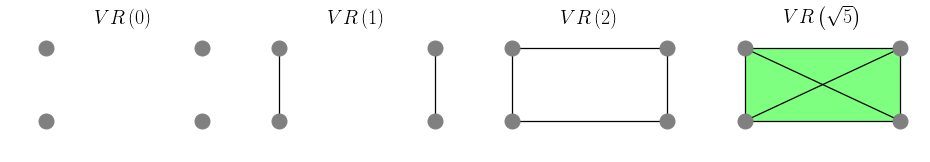
\includegraphics[width=3.75in]{figures/vrcomplex-diagram.png}
%
\label{fig:vrcomplex-diagram}
\end{figure}
%

\subsection{Using vectorized persistence homology representations for cancer grading}
\label{sec:method:proposed}

\section{Results}
\label{results}
We used the MICCAI 2015 Gland Segmentation Challenge Contest dataset~\cite{Sirinukunwattana2017} to develop and validate the proposed method. This dataset contains a total of 165 images derived from 16 hematoxylin-eosin stained histological sections of stage T3 and T4 colorectal adenocarcinoma digitized using a Zeiss MIRAX MIDI SlideScanner with a pixel resolution of $0.620 \mu m$ equivalent to a 20x objective magnification. An expert pathologist delineated the boundary of all the glands in each image and graded the image as either $benign$ or $malignant$ based on the overall glandular architecture. Figure 1 shows representative example images of the two grades and Table 1 shows the distribution of grades in the training and testing sets.

% References
\bibliographystyle{IEEEbib}
\bibliography{mendeley}

\end{document}
